\chapter{Optimización}
\label{cap:optimizacion}

\section{Optimalidad local y global}

\begin{definicion}
Sea $f:\R^d\to\R$. Un punto $\theta^\star$ es un \emph{mínimo global} si $f(\theta^\star)\le f(\theta)$ para todo $\theta$, y un \emph{mínimo local} si existe $\varepsilon>0$ tal que $f(\theta^\star)\le f(\theta)$ para todo $\theta$ con $\|\theta-\theta^\star\|<\varepsilon$.
\end{definicion}

\paragraph{Condiciones de optimalidad.} Si $f$ es dos veces diferenciable y $\theta^\star$ es un mínimo local, entonces $\nabla f(\theta^\star) = 0$ (primer orden) y $\nabla^2 f(\theta^\star)\succeq 0$ (segundo orden necesaria). Si $\nabla f(\theta^\star) = 0$ y $\nabla^2 f(\theta^\star)\succ 0$, entonces $\theta^\star$ es un mínimo local estricto (segundo orden suficiente) \parencite[cap.~2]{nocedal2006}.

\section{Convexidad}

\begin{definicion}
$f$ es convexa si $f(\alpha\theta + (1-\alpha)\theta')\le\alpha f(\theta)+(1-\alpha)f(\theta')$ para todo $\theta,\theta'$ y $\alpha\in[0,1]$, y estrictamente convexa si la desigualdad es estricta cuando $\theta\ne\theta'$ y $\alpha\in(0,1)$.
\end{definicion}

\begin{teorema}\label{teo:local_global}
Si $f$ es convexa, todo mínimo local es global. Si además es estrictamente convexa, el mínimo global (si existe) es único.
\end{teorema}
\begin{proof}
Sea $\theta^\star$ un mínimo local y supóngase que existe $\theta'$ con $f(\theta') < f(\theta^\star)$. Para $\alpha\in(0,1]$, $f(\theta^\star + \alpha(\theta'-\theta^\star)) \le (1-\alpha)f(\theta^\star) + \alpha f(\theta') < f(\theta^\star)$. Tomando $\alpha$ suficientemente chico, el punto queda dentro de cualquier entorno de $\theta^\star$, lo que contradice que sea mínimo local. Para la unicidad: si $\theta_1\ne\theta_2$ fueran dos mínimos globales con valor $f^\star$, por convexidad estricta $f(\tfrac12\theta_1+\tfrac12\theta_2)<f^\star$, absurdo.
\end{proof}

\begin{proposicion}\label{prop:logistica_convexa}
La pérdida logística regularizada
\[
f(\bm w,b) = \frac1n\sum_i c_i\big[\log(1+e^{z_i}) - y_i z_i\big] + \frac\mu2\|\bm w\|^2,\qquad z_i = \bm w^\top\bm x_i + b,\ c_i>0,
\]
es convexa en $(\bm w, b)$, y estrictamente convexa en $\bm w$ si $\mu > 0$.
\end{proposicion}
\begin{proof}
Con $\tilde{\bm x}_i = (\bm x_i, 1)$, el gradiente es $\nabla f = \frac1n\sum_i c_i(\sigma(z_i) - y_i)\tilde{\bm x}_i + \mu(\bm w,0)$ y el Hessiano
\[
\nabla^2 f = \frac1n \tilde X^\top D\tilde X + \mu\begin{pmatrix} I & 0\\ 0 & 0\end{pmatrix},\qquad D = \operatorname{diag}\big(c_i\,\sigma(z_i)(1-\sigma(z_i))\big).
\]
Como $D$ tiene diagonal positiva, $\bm v^\top\tilde X^\top D\tilde X\bm v = \sum_i D_{ii}(\tilde{\bm x}_i^\top\bm v)^2\ge 0$, y el término de regularización suma $\mu\|\bm v_{\bm w}\|^2 > 0$ para toda dirección con componente no nula en $\bm w$.
\end{proof}

En cambio, la pérdida de una red con al menos una capa oculta no es convexa: basta observar que permutar las unidades de una capa oculta da otra red con exactamente la misma salida, de modo que si $\theta^\star$ es un mínimo con unidades distintas, sus permutaciones son mínimos distintos con el mismo valor, y por el teorema~\ref{teo:local_global} una función estrictamente convexa no puede tenerlos. Por eso, en el caso no convexo, el punto de llegada depende de la inicialización y del optimizador (hipótesis~\ref{h:noconvexo}).

\section{Descenso por gradiente}

\pendiente{tasa de convergencia para $f$ $L$-suave y $\mu$-fuertemente convexa: $f(\theta_t)-f^\star\le(1-\mu/L)^t(f(\theta_0)-f^\star)$; número de condición.}

\section{Descenso por gradiente estocástico}

\pendiente{estimador insesgado del gradiente; con tasa constante, SGD converge a una vecindad de $\theta^\star$ de tamaño $O(\eta)$, lo que explica la brecha observada en la figura~\ref{fig:convexo}.}

\section{Momento y aceleración de Nesterov}

\pendiente{ecuaciones de momento clásico y de Nesterov \parencite{sutskever2013}; interpretación como bola pesada.}

\section{Métodos adaptativos: RMSProp, Adam y AdamW}

\pendiente{ecuaciones de RMSProp \parencite{tieleman2012}, Adam con corrección de sesgo \parencite{kingma2015} y AdamW \parencite{loshchilov2019}; discusión de \textcite{wilson2017}.}

\section{Métodos cuasi-Newton: L-BFGS}

\pendiente{paso de Newton, condición de secante, actualización BFGS, memoria limitada, búsqueda lineal con condiciones de Wolfe fuertes \parencite{liu1989,nocedal2006}.}

\section{El método del simplex de Nelder-Mead}

\pendiente{operaciones de reflexión, expansión, contracción y encogimiento sobre un simplex de $d+1$ vértices \parencite{nelder1965}; no usa derivadas; costo y falta de garantías de convergencia en dimensión alta.}

\begin{figure}[ht]
\centering
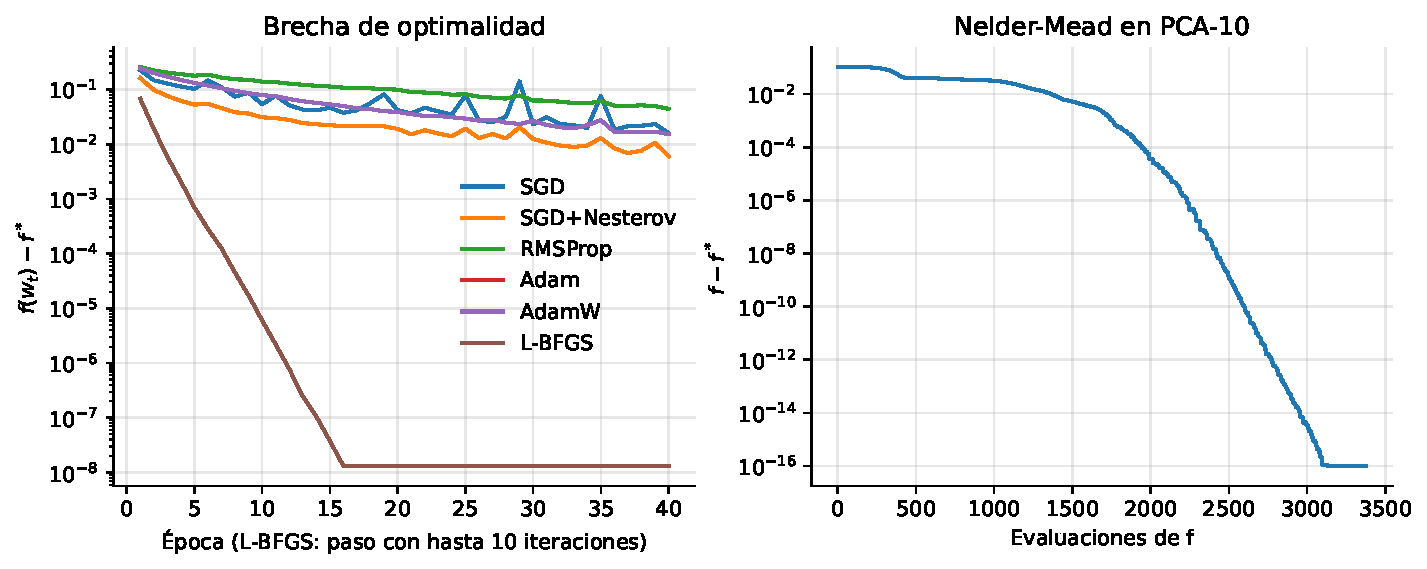
\includegraphics[width=\linewidth]{convexo_brecha}
\caption{Brecha de optimalidad $f(w_t)-f^\star$ en la regresión logística regularizada (izquierda) y de Nelder-Mead en un subespacio de 10 dimensiones (derecha).}
\label{fig:convexo}
\end{figure}
